\chapter{HDF4 Data Files}
HDF4 (Hierarchical Data Format version 4) was chosen by the CALIPSO, CloudSat
and MODIS missions as the primary file format for storage and distribution of
down-linked scientific and ancillary data. It is a self-describing,
platform-independent binary format designed for storage of large data sets and
metadata, encapsulated together in a single file. Objects that can be contained
in an HDF file include multi-dimensional arrays (`Scientific Data Set' or
`SDS'), tables (`Vdata'), raster images, palettes and
annotations organised hierarchically in groups (`Vgroup'). Each object as
well as the file itself can further be described by an arbitrary number of
name-value pairs (`attribute').

Numerous NASA EOS missions, such as CloudSat and MODIS, use an extended version
of HFD4 called HDF-EOS2, described later in this chapter.

HDF4 API (Application Programming Interface) is available
for FORTRAN-77 and C, although various other languages are supported through
third-party libraries. Additionally, a vast number of tools for manipulating
these formats exist. A list such tools can be found on the web site of the \textit{HDF Group}
[\url{http://www.hdfgroup.org}] and the \textit{HDF-EOS Tools and
Information Center} [\url{http://www.hdfeos.org/}]. In particular,
\textit{HDFView} is
a convenient GUI application for examining HDF4 files.

\begin{figure}[h]
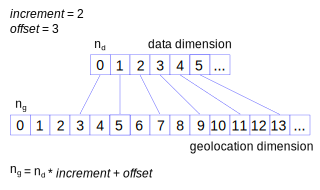
\includegraphics[width=200pt]{images/dimension-mapping.pdf}
\caption[Dimension mapping example]{\textbf{Dimension mapping example.} \textit{Swath} data type allows
indices of
geolocation dimension and its associated data dimension to be in none-1:1
relationship. Geo-indices $n_g$ are translated to data-indices $n_d$ by
multiplying by \textit{increment} and adding \textit{offset}.}
\label{fig:dimension-mapping}
\end{figure}


\begin{table}[h]
\caption[Attributes predefined by HDF4]{\textbf{Attributes predefined by HDF4.} Many product files do not
follow the
specification closely or invent their own attributes with a similar meaning (see
footnotes). Note that this is not a full list of predefined attributes.}
\label{tab:hdf4-attributes}
\begin{tabularx}{\textwidth}{llXl}
  \sffamily{\textbf{Data Object}}
& \sffamily{\textbf{Attribute Name}}
& \sffamily{\textbf{Description}}
& \sffamily{\textbf{Example}}\\
\tophline

SDS/dimension
& long\_name
& Name of the array.
& Gaseous\_Attenuation\\

SDS/dimension
& units
& Physical units of object items.
& dBZe\\

SDS
& valid\_range
& Minimum and maximum values. & 0,1000\mpfootnotemark[1]\\

SDS
& \_\_FillValue\mpfootnotemark[2]
& Value used to fill empty array items (expected, but did not appear).
& 65535\\

SDS
& scale\_factor\mpfootnotemark[3]
& Value by which each array item is to be multiplied.
& 100.0\\

SDS
& add\_offset\mpfootnotemark[3]
& Value to add to each array item.
& 0.0\\

SDS
& missing\_value\mpfootnotemark[4]
& Value used to fill empty array items (never expected to be filled).
& -9999
\end{tabularx}

\footnotetext[1]{CALIPSO products denote valid\_range as `<min>....<max>'.}
\footnotetext[2]{In CALIPSO products, this attribute is called
\textit{fillvalue}.}
\footnotetext[3]{Values in SDS can be scaled and shifted for space efficiency. In
CloudSat products, these are called \textit{factor} and \textit{offset}.}
\footnotetext[4]{In CloudSat products, this attribute is called
\textit{missing}; additionally, attribute \textit{missop} specifies operator
(`<', `<=', `==', `>=', or `>') to be used for comparison of data items with
\textit{missing}.}
\end{table}

\section{Multi-dimensional Arrays, Dimensions and Attributes}
Every SDS is associated with a number of dimensions, each of a particular
\textit{size} (or, in a special case, unlimited size). In HDF4 context, the
number of dimensions of an array is called the \textit{rank}. Array indices are
counted from zero, and range up to \textit{size}-1 (incl.). Dimensions can
optionally be named. HDF4 standardises some predefined SDS and dimension
attributes (Tab.\,\ref{tab:hdf4-attributes}).

\section{HDF-EOS2}\label{sec:hdf-eos2}
HDF-EOS2 is an extension to HDF4, which defines three new \textit{data types}
based on regular HDF4 structures, designed to accommodate data sets commonly
produced by earth-observing missions: 

\begin{enumerate}
\item Swath --- time-ordered data such as series of scanlines or series of
profiles (Fig.\,\ref{fig:swath}).
\item Grid --- data geolocated on a rectilinear grid.
\item Point --- sparsely geolocated data, such as records from ground stations.
\end{enumerate}

\begin{figure}[h]
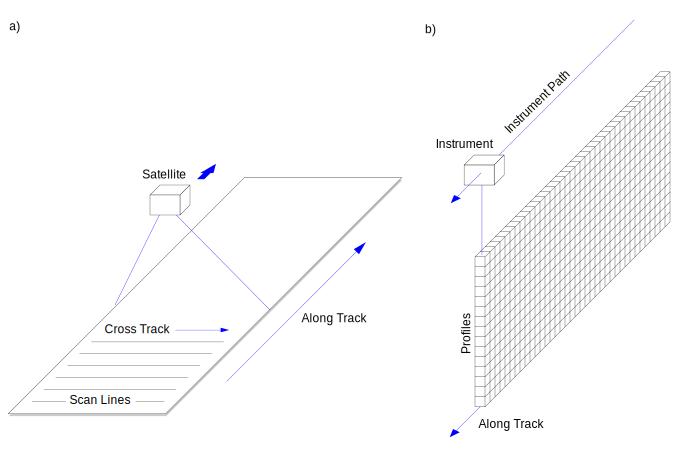
\includegraphics[width=\textwidth]{images/swath.pdf}
\caption[HDF-EOS2 swath]{\textbf{HDF-EOS2 swath.} Swath is typically deployed to store
data from a \textbf{a},
scanning instrument, \textbf{b}, profiling instrument. [Adapted from
\cite{HDF_EOS_UsersGuideVol1_2009}.]}
\label{fig:swath}
\end{figure}

\begin{figure}[h]
\raggedright
\sffamily{a)}

\includegraphics[width=\textwidth]{images/calipso-file-naming.pdf}
%\rule{\linewidth}{0.3pt}
\sffamily{b)}
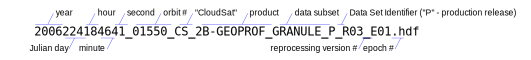
\includegraphics[width=\textwidth]{images/cloudsat-file-naming.pdf}
%\rule{\linewidth}{0.3pt}
\sffamily{c)}

\includegraphics[width=\textwidth]{images/modis-file-naming.pdf}
\caption[File naming conventions]{\textbf{File naming conventions.} \textbf{a}, CALIPSO, \textbf{b}, CloudSat, \textbf{c}, MODIS
(based on \url{http://modis-atmos.gsfc.nasa.gov/products_filename.html}). }
\label{fig:file-naming}
\end{figure}

Fields in HDF-EOS2 files are separated in \textit{Geolocation Fields} and
\textit{Data Fields} groups. Fields, dimensions and relations between
geolocation and data fields are described in the \textit{HDF-EOS2 metadata}. Internally,
this metadata information is stored as a continuous block of text inside the HDF4
file attribute \textit{StructMetadata.0}, and encoded as PVL (Parameter Value
Language), a markup language similar to XML. HDF-EOS2 library provides functions
to access this information directly, effectively hiding the underlying structure
from the programmer, and therefore alleviates the need to parse the language.

HDF-EOS2 files of MODIS contain another metadata structure --- \textit{ECS Core
Metadata} stored in the \textit{CoreMetadata.0} file attribute, similar to \textit{StructMetadata.0}. Its aim is to provide information on spatial
and temporal coverage, data quality and production status for searching
purposes. \textit{ECS Core Metadata} can be read with the \textit{SDP Toolkit}
available
through the \textit{HDF-EOS Tools and Information Center}
[\url{http://www.hdfeos.org/}].


\subsection{Dimension Mapping}
\textit{Swath data type} provides an optional feature called \textit{dimension mapping}, which
allows geolocation fields to have lower resolution than corresponding data
fields. If dimension mapping is used, one has to distinguish between
\textit{geolocation
dimensions} and \textit{data dimensions}. The relationship between geolocation
and data
dimensions is linear, defined by two constants: \textit{offset} and
\textit{increment}. Reversed dimension mapping, i.e. data fields of lower
resolution than geolocation fields is also supported, although its
applicability is likely to be not as high. The principle is illustrated in
Fig.\,\ref{fig:dimension-mapping}.


\section{CALIPSO Products}\label{sec:hdf-calipso-products}
CALIPSO mission deploys HDF4 format for product distribution. File naming
convention is explained in Fig.\,\ref{fig:file-naming}. Generally,
these products come in two kinds: profile products and layer products, as
described in Section\,\ref{sec:calipso-data-products}\,.
The structure of CALIPSO products is flat; no explicit distinction is made
between
geolocation and data fields. Dimensions do not possess any explicitly meaningful
names.

Let us consider the \textbf{333-m Lidar Level 2 Cloud and Aerosol Layer Product}
as an
example (Fig.\,\ref{fig:hdf4-calipso}). One-dimensional arrays
\textbf{\textit{Latitude}}\,[63120], \textbf{\textit{Longitude}}\,[63120]
and \textbf{\textit{Profile\_UTC\_Time}}\,[63120] locate data sets spatially
and temporally. In contrast with profile products, layer products are a
expressed
as a sequence of columns (in the along-scan direction) composed of 0-5 layers
each. Number of layers in columns is stored in a one-dimensional array
\textbf{\textit{Number\_Layers\_Found}}\,[63120]. Base and top altitudes of the
layers found are stored in two-dimensional arrays
\textbf{\textit{Layer\_Top\_Altitude}}\,[63120\,\texttimes\,5] and
\textbf{\textit{Layer\_Base\_Altitude}}\,[63120\,\texttimes\,5]. Finally, the
actual data can be found in a two-dimensional
array
\textbf{\textit{
Integrated\_Attenuated\_Backscatter\_532}}\,[63120\,\texttimes\,5],
 and in a number of other fields.

\section{CloudSat Products}
Data from the CloudSat mission are commonly distributed in per-granule HDF-EOS2
files. File naming convention is described in
Fig.\,\ref{fig:file-naming}. The 2B-GEOPROF product contains a single swath
called \textit{2B-GEOPROF}. Two important dimensions are \textit{nray}, which is the
horizontal dimension (number of profiles), and \textit{nbin}, which is the
vertical dimension (number of bins). Data fields such as
\textbf{\textit{Gaseous\_Attenuation}}\,[nray\,\texttimes \,nbin] are
two-dimensional arrays, located spatially by one-dimensional arrays
\textbf{\textit{Latitude}}\,[nray],
\textbf{\textit{Longitude}}\,[nray]
and \textbf{\textit{Height}}\,[nray\,\texttimes\,nbin] and
temporally by \textbf{\textit{Profile\_time}}\,[nray]
(Fig.\,\ref{fig:hdfeos2-2bgeoprof}).
Time corresponding to a particular ray is calculated by adding
\textbf{\textit{Profile\_time}} to \textbf{\textit{start\_time}} (in UTC). The
result is time in UTC, although it may differ from the proper UTC time in the
rare event when a leap second is introduced in the time period covered by the
granule.
Other CloudSat products resemble a similar
structure. Comprehensive documentation of the products can be found on the
CloudSat DPC web site [\url{http://www.cloudsat.cira.colostate.edu/}].


\section{Aqua MODIS Level 1B Products}
There are three Aqua MODIS Level 1B products: MYD02QKM, MYD02HKM and
MYD021\-KM, described in detail in Section\,\ref{sec:modis-level1b-data-products}\,.
They are distributed in
HDF-EOS2
format. Every granule is either a `\textit{day mode}' , `\textit{night mode}', or a `\textit{mixed mode}'
granule, depending on whether it contains RefSB bands on the entire swath, none
of it, or a fraction of it (resp.). File naming convention employed by MODIS is
described in Fig.\,\ref{fig:file-naming}.

Let us now consider a day mode MYD02QKM product as an example
(Fig.\,\ref{fig:hdfeos2-modis}). The
HDF-EOS2 file contains a single swath
called \textbf{\textit{MODIS\_SWATH\_Type\_L1B}}. Geolocation dimensions are
\textit{Max\_EV\_Frames} and \textit{10*nscans}. Their corresponding data
dimensions are
\textit{4*Max\_EV\_Frames} and \textit{40*nscans}. As you can see in
Fig.\,\ref{fig:hdfeos2-modis}, MODIS products
utilise dimension mapping, so that geolocation fields can be specified more
sparsely than data fields. \textbf{\textit{Ge\-o\-lo\-ca\-ti\-on Fields}} group contains
two two-dimensional
arrays: \textbf{\textit{Latitude}}\,[10*nscans\,\texttimes\,Max\_EV\-\_frames] and
\textbf{\textit{Longitude}}\,[10*nscans\,\texttimes\,Max\_EV\_frames].
\textbf{\textit{Data Fields}}
group contains a three-dimen\-sional array
\textbf{\textit{EV\_250\_RefSB}}\,[Band\_250M\,\texttimes\,40*nscans\,
\texttimes\ ,
4*Max\_EV\_frames] with the actual data. The dimension
\textit{Band\_250M} is of size 2, because there are only two bands in this band
grouping (see Tab.\,\ref{tab:bands} in the previous chapter).

\section{More Information}
Much of the information in this chapter is based on the following documents:

\begin{itemize}
\item \cite{HDF_EOS_UsersGuideVol1_2009}
\item \cite{HDF_42r4UsersGuide2009}
\item \cite{CALIPSO_Catalog2007}
\item \cite{CloudSatHandbook2008}
\item CloudSat DPC web product documentation
at \url{http://www.cloudsat.cira.colostate.edu/dataSpecs.php}
\item \cite{MODIS_Level1B_ProductUsersGuide2009}
\end{itemize}

\begin{figure}[p]
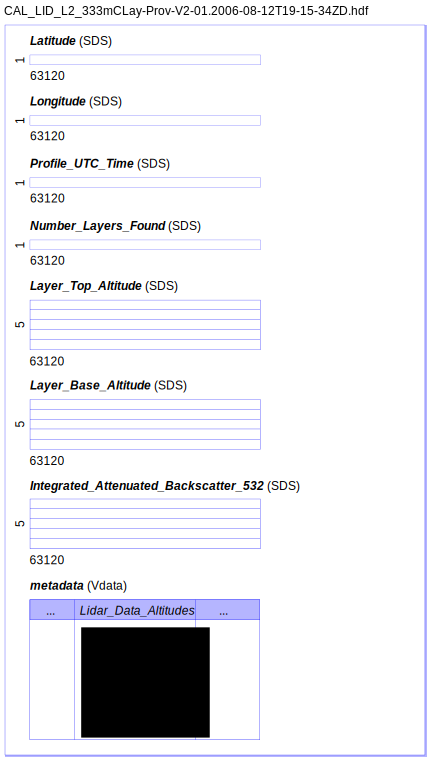
\includegraphics[width=300pt]{images/hdf4_calipso.pdf}
\caption[CALIPSO HDF4 diagram]{\textbf{CALIPSO HDF4 diagram.} This is the structure of a typical
CALIPSO Level~2 Layer Product. Note that
\textbf{\textit{metadata}} is the name of a Vdata object, and does not tally
with the term `\textit{metadata}' used elsewhere in this document, which refers to HDF4
attributes. Although the \textit{Lidar\_Data\_Altitudes} field of the
\textbf{\textit{metadata}} table is not particularly relevant for \textit{layer} products,
it provides the only means how one can retrieve height
information, essential for plotting \textit{profile} products.}
\label{fig:hdf4-calipso}
\end{figure}

\begin{figure}[p]
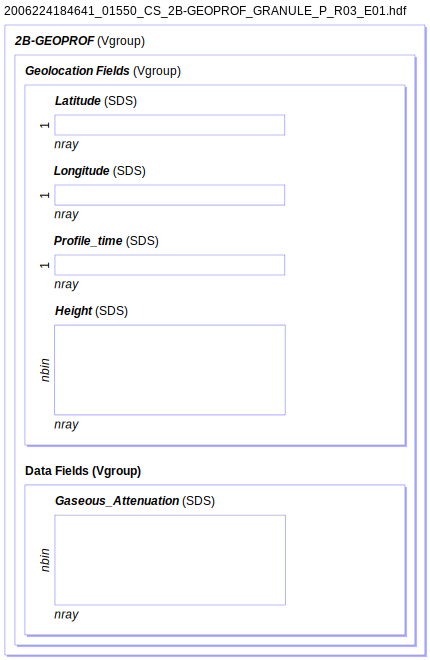
\includegraphics[width=300pt]{images/hdf-eos2_2b-geoprof.pdf}
\caption[CloudSat 2B-GEOPROF HDF-EOS2 diagram]{\textbf{CloudSat 2B-GEOPROF HDF-EOS2 diagram.}
This is the structure a typical CloudSat 2B-GEOPROF product.}
\label{fig:hdfeos2-2bgeoprof}
\end{figure}

\begin{figure}[p]
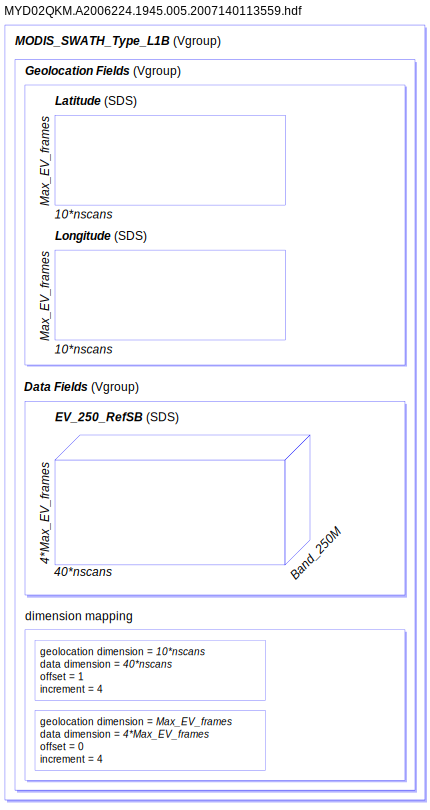
\includegraphics[width=300pt]{images/hdf-eos2_modis.pdf}
\caption[MODIS Level 1B HDF-EOS2 diagram]{\textbf{MODIS Level 1B HDF-EOS2 diagram.} This is the structure of a
typical MODIS Level~1B product.}
\label{fig:hdfeos2-modis}
\end{figure}
